\section{Results}\label{sec:results}

The system was tested with 80 test images (overview of banknotes value distribution shown in \cref{tab:dataset-overview}) that contained banknotes in the most common conditions, such as different perspective views, cluttered environments, partially occluded banknotes and also multiple banknotes per image (67 images had only 1 banknote, 11 images had 2 banknotes and 2 images had 3 banknotes). 

With the proper selection of the keypoint detection and description algorithm (depending on the image contents), the system successfully recognized all the 95 banknotes in the 80 test images. The most successful configurations are shown in \cref{tab:recognition-configurations}, which was built by manually inspecting each test image recognition results and selecting the configuration which successfully recognized all banknotes in the image and achieved better contour estimation.

In \cref{fig:recognition-clutter,fig:recognition-perspective-distortion,fig:recognition-partially-occluded-banknotes,fig:recognition-overlapping-banknotes} are shown some representative results of the implemented banknote recognition system, showing detection of banknotes with background clutter, perspective distortion, folding and partial occlusion.


\begin{table}[ht]
	\centering
	\caption{Testing dataset overview}
	\begin{tabu} to 0.47\textwidth { X[4.5,l,m] X[0.6,l,m] X[0.8,l,m] X[0.8,l,m] X[0.8,l,m] X[l,m] X[l,m] X[l,m] }
		\textbf{Banknote value} & 5\,\euro{} & 10\,\euro{} & 20\,\euro{} & 50\,\euro{} & 100\,\euro{} & 200\,\euro{} & 500\,\euro{}	\\
		\noalign{\vskip 1mm}
		\hline
		\noalign{\vskip 1mm}
		\textbf{Nº of banknotes}			& 15		 & 12		   & 19			 & 19		   & 6			  & 9			 & 15			\\
	\end{tabu}
	\label{tab:dataset-overview}
\end{table}


\begin{table}[ht]
	\caption{Selection of the configurations with the best recognition results (1 configuration per test image)}
	\centering
	\begin{tabu} to 0.47\textwidth { X[0.6,c,m] X[0.8,c,m] X[c,m] X[c,m] X[c,m] }
		\rowfont{\bfseries\itshape} Detector & Descriptor & Images with 1 banknote & Images with 2 banknotes & Images with 3 banknotes \\
		\noalign{\vskip 2mm}
		\hline
		\noalign{\vskip 2mm}
		SIFT	 & SIFT		  & 37			   & 7				  & 2	\\
		SURF	 & SURF		  & 24			   & 3				  & 0	\\
		GFTT	 & SIFT		  & 3			   & 1				  & 0	\\
		FAST	 & SIFT		  & 1			   & 0				  & 0	\\
		BRISK	 & BRISK	  & 1			   & 0				  & 0	\\
		ORB		 & ORB		  & 1			   & 0				  & 0	\\
	\end{tabu}
	\label{tab:recognition-configurations}
\end{table}


\begin{figure}[H]
	\centering
	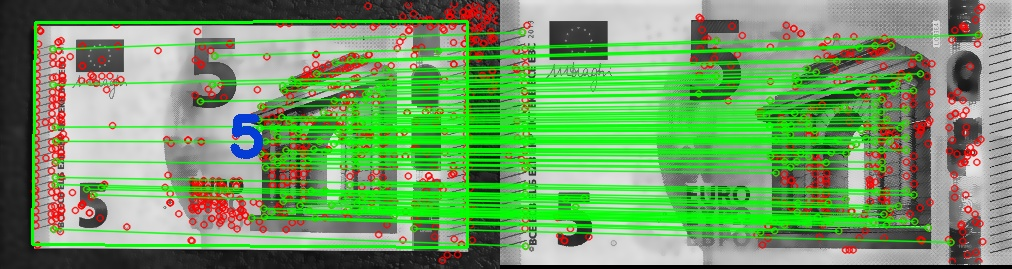
\includegraphics[width=0.36\textwidth]{notes-recognition/5__(5).jpg___SIFT-Detector_SIFT-Extractor_BF-Matcher_lowQualityImageDB_globalMatch__inliersMatches__0}\hfill
	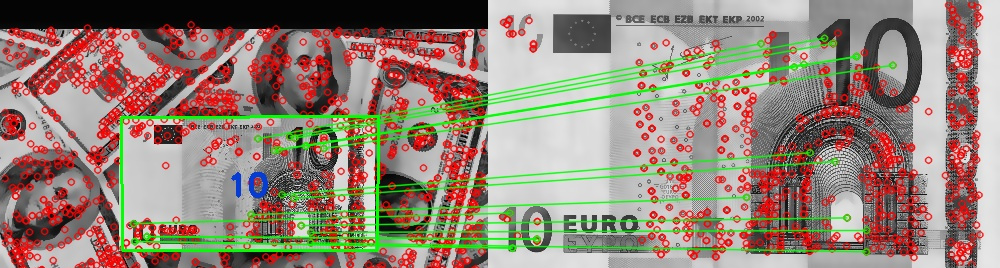
\includegraphics[width=0.36\textwidth]{notes-recognition/10__(9).jpeg___SIFT-Detector_SIFT-Extractor_BF-Matcher_lowQualityImageDB_globalMatch__inliersMatches__0}
	\caption{Detection of a banknote in an ideal perspective view with (bottom) and without (top) background clutter (using SIFT detector, SIFT descriptors and BFMatcher)}
	\label{fig:recognition-clutter}
\end{figure}

\begin{figure}[H]
	\centering
	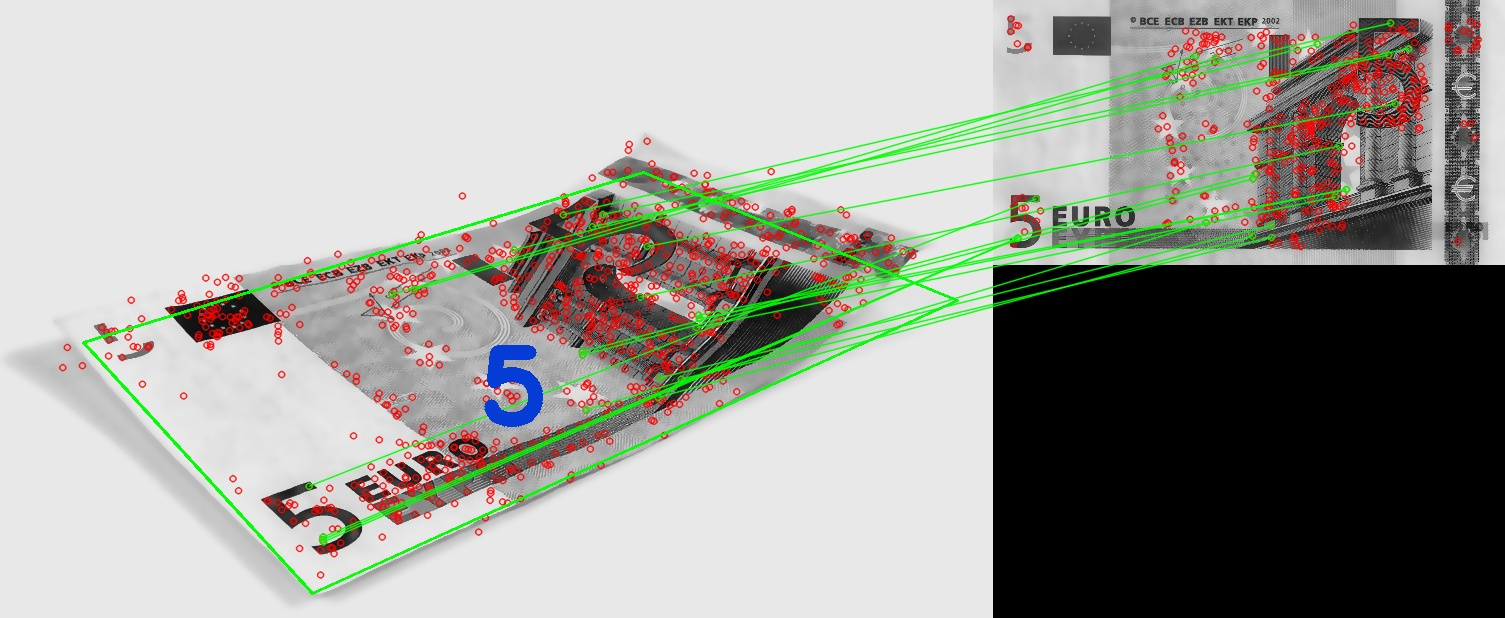
\includegraphics[width=0.36\textwidth]{notes-recognition/5__(6).jpg___SURF-Detector_SURF-Extractor_BF-Matcher_lowQualityImageDB_globalMatch__inliersMatches__0}\hfill
	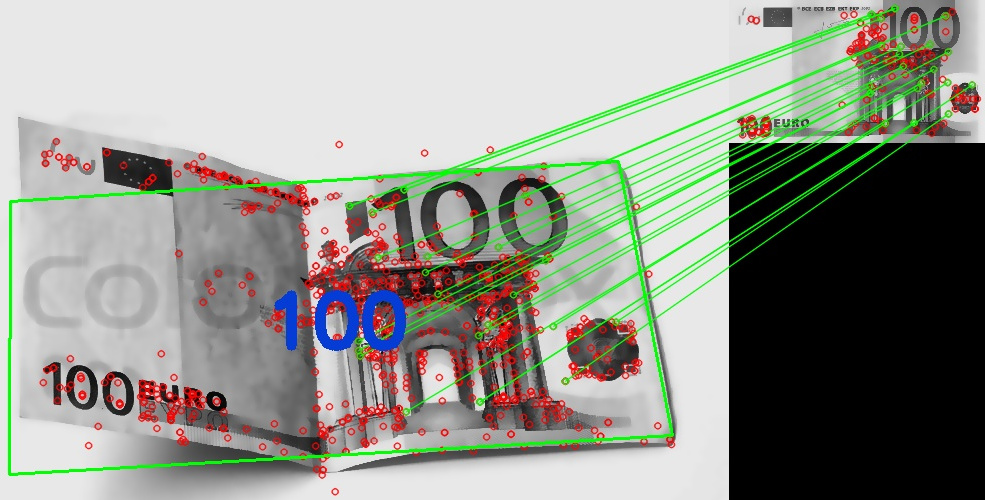
\includegraphics[width=0.36\textwidth]{notes-recognition/100__(4).jpg___SIFT-Detector_SIFT-Extractor_BF-Matcher_dynamicQualityImageDB_globalMatch__inliersMatches__0.jpg}
	\caption{Detection of banknotes with perspective distortion and folding (left image used SURF detector, SURF descriptors and BFMatcher while the right image used SIFT detector, SIFT descriptors and BFMatcher)}
	\label{fig:recognition-perspective-distortion}
\end{figure}


\begin{figure}[H]
	\centering
	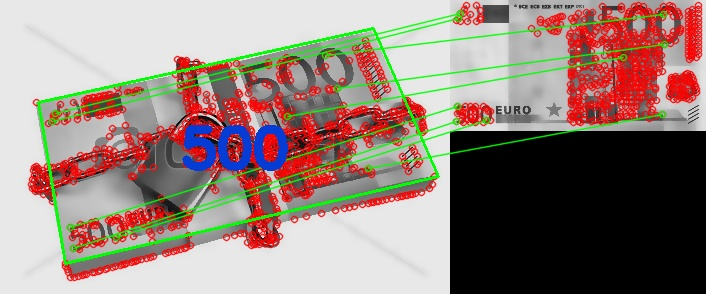
\includegraphics[width=0.405\textwidth]{notes-recognition/500.jpg___GFTT-Detector_SIFT-Extractor_BF-Matcher_dynamicQualityImageDB_globalMatch__inliersMatches__0}\hfill
	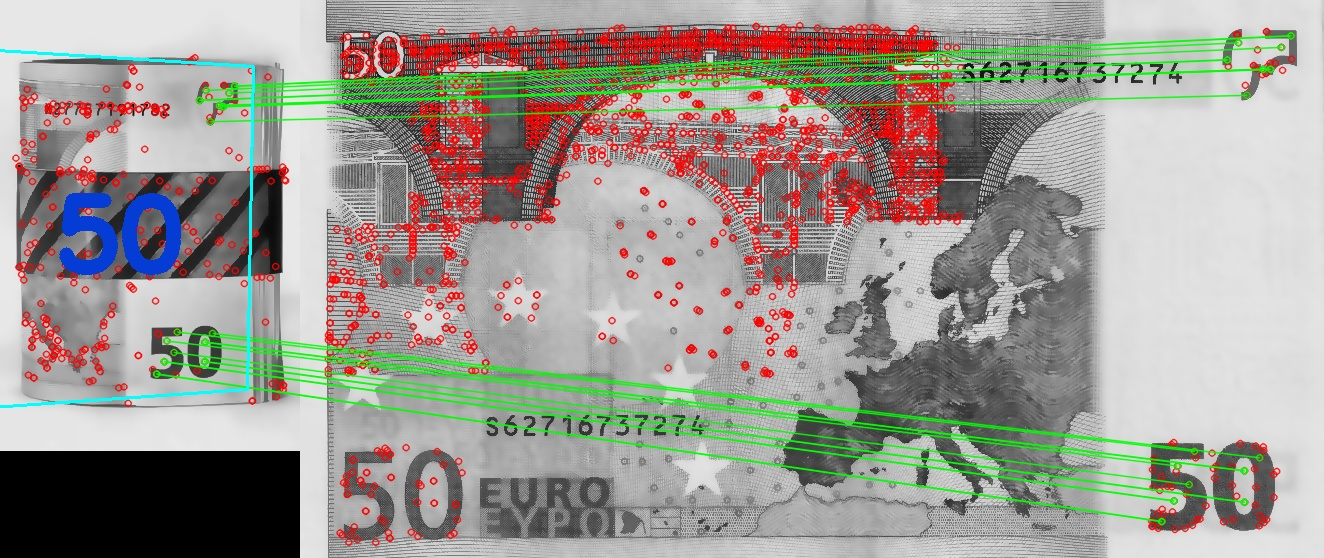
\includegraphics[width=0.405\textwidth]{notes-recognition/50__(13).jpg___SIFT-Detector_SIFT-Extractor_BF-Matcher_mediumQualityImageDB_globalMatch__inliersMatches__0}
	\caption{Detection of partially occluded banknotes (left image used GFTT detector, SIFT descriptors and BFMatcher while the right image used SIFT detector, SIFT descriptors and BFMatcher)}
	\label{fig:recognition-partially-occluded-banknotes}
\end{figure}

\begin{figure}[H]
	\centering
	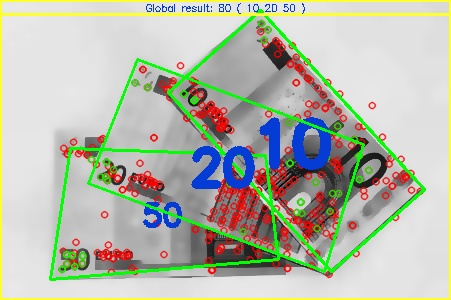
\includegraphics[width=0.405\textwidth]{notes-recognition/10-20-50.jpg___SIFT-Detector_SIFT-Extractor_BF-Matcher_dynamicQualityImageDB_globalMatch}
	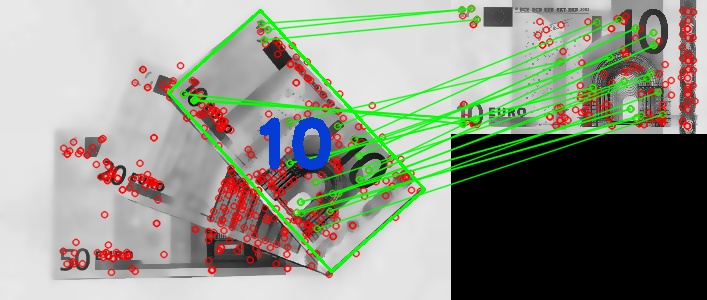
\includegraphics[width=0.405\textwidth]{notes-recognition/10-20-50.jpg___SIFT-Detector_SIFT-Extractor_BF-Matcher_dynamicQualityImageDB_globalMatch__inliersMatches__1}
	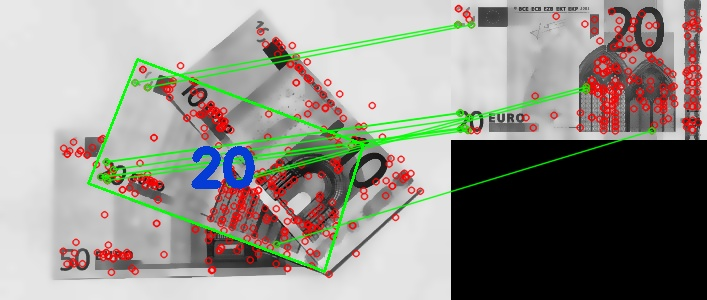
\includegraphics[width=0.405\textwidth]{notes-recognition/10-20-50.jpg___SIFT-Detector_SIFT-Extractor_BF-Matcher_dynamicQualityImageDB_globalMatch__inliersMatches__2}
	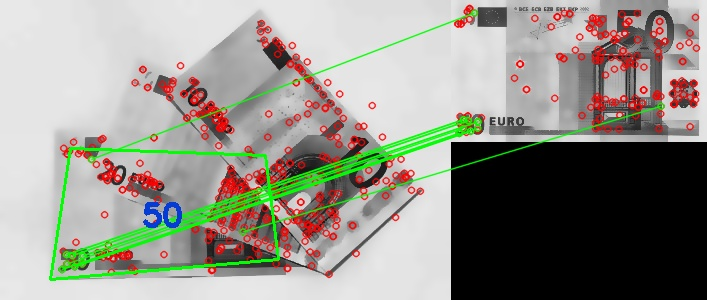
\includegraphics[width=0.405\textwidth]{notes-recognition/10-20-50.jpg___SIFT-Detector_SIFT-Extractor_BF-Matcher_dynamicQualityImageDB_globalMatch__inliersMatches__0}
	\caption{Detection of overlapping banknotes (using SIFT detector, SIFT descriptors and BFMatcher)}
	\label{fig:recognition-overlapping-banknotes}
\end{figure}
